\documentclass[a4paper]{scrreprt}

\usepackage[utf8]{inputenc}
\usepackage[T1]{fontenc}
\usepackage[colorlinks=true]{hyperref}
\usepackage{graphicx}
\usepackage{listings}
\usepackage{pdflscape}
\usepackage{rotating}
\usepackage{afterpage}

\lstdefinestyle{BashStyle}{
  language=bash,
  basicstyle=\small\ttfamily,
  %numbers=left,
  %numberstyle=\tiny,
  %numbersep=3pt,
  frame=tb,
  columns=fullflexible,
  %backgroundcolor=\color{yellow},
  linewidth=0.9\linewidth,
  xleftmargin=0.1\linewidth
}

\title{Building for the ARM Cortex-M0 with GNU tools}
\author{James Gowans}

\begin{document}

\maketitle
\section*{Licence}
This work is licensed under the Creative Commons Attribution-ShareAlike 3.0 Unported License. To view a copy of this license, visit http://creativecommons.org/licenses/by-sa/3.0/ or send a letter to Creative Commons, 444 Castro Street, Suite 900, Mountain View, California, 94041, USA.

\section*{Preface}
This guide is intended for a range of audiences from those who have never compiled code with GCC before, to those who are experienced with GNU and want to start writing code for ARM.
This guide does not intend to teach you programming, only building and debugging. You should have some familiarity with C and assembly before attempting to develop code.

\tableofcontents

\newpage
\chapter{Toolchain Overview}
\afterpage{
\begin{landscape}
\begin{figure}
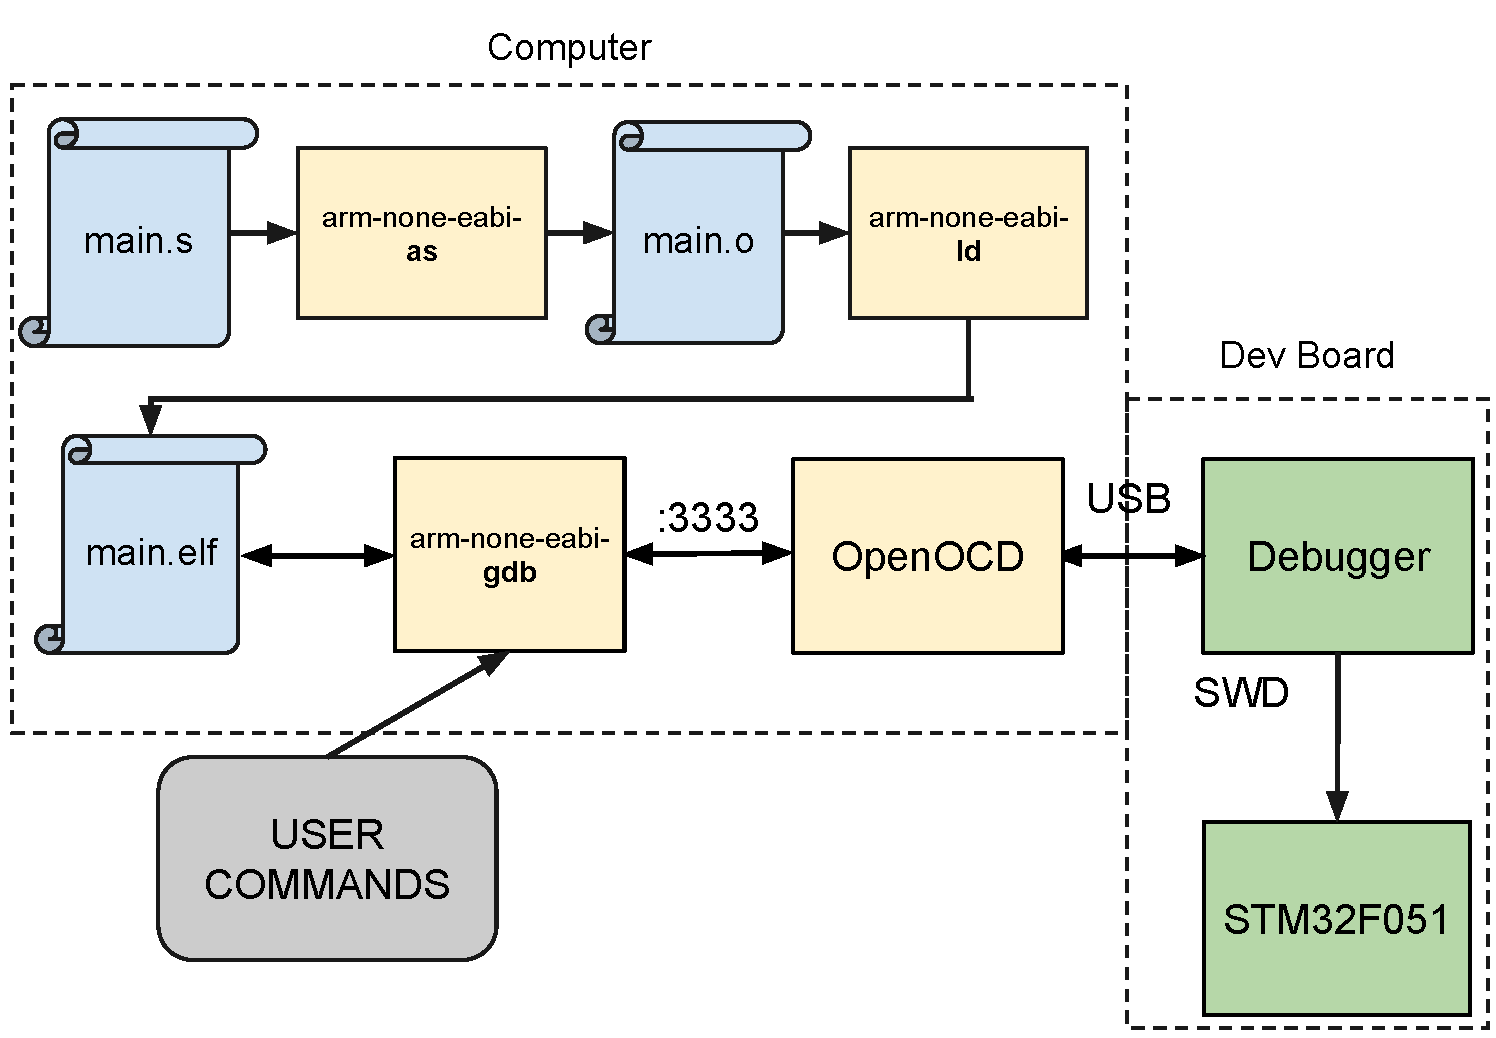
\includegraphics[width=1.4\textwidth]{./img/assembly_to_micro_process.pdf}
\caption{Process which source files takes to be loaded onto micro.}
\label{fig:assembly_to_micro_proc}
\end{figure}
\end{landscape}
}
A toolchain is a collection of software tools that facilitates the process of getting your source code executing on a target platform. This guide will start with the simplest toolchain and introduce more tools and complexity later as required. The simplest set of tools is shown graphically in \autoref{fig:assembly_to_micro_proc} and will now be discussed.

\begin{enumerate}
\item \emph{Text editor:} provides the capability to modify source code files. Typically something like notepad (Windows) or gedit (Linux) will work fine. However, it's recommended for Windows users to install a more customisable editor: Notepad++
\item \emph{Assembler:} converts human-readable assembly code into relocatable (no final address) machine code files. These files are known as object files and are not directly executable. 
\item \emph{Linker:} takes one or more object files and turns them into a single executable which can run directly on the target. The process of linking involves ascertaining the final (absolute) memory address for each section of the executable.
\item \emph{OpenOCD} (On Chip Debugger). This is an interface to the hardware debugger. The hardware debugger microcontroller will typically be connected to the computer via a USB connection. There needs to be a way to send data down the USB cable to the debugger to get it to load code onto the micro or debug running code.
When running in Windows, the ST-Link driver is required. When running in Linux the libusb-1.0 package is required. 
\item \emph{GDB} (GNU debugger) This is a debugger client. It is software which connects to the hardware debugger through the interface and manages what the hardware debugger does by sending it instructions. This can involve sending it executable machine code to load onto the target microcontroller, or causing the target to stop/start/pause execution of the code, or even reading/writing of data in the memory of the target. 
\end{enumerate}

The is a software package called gcc-arm-none-eabi which provides the assembler (arm-none-eabi-as), the linker (arm-none-eabi-ld) as well as the debugger (arm-none-eabi-gdb). 
We will now proceed to review gcc-arm-none-eabi and OpenOCD in some detail.

\section{gcc-arm-none-eabi}
gcc-arm-none-eabi is a fork of the very popular GCC, developed by GNU. This particular fork is maintained by the guys at ARM so it's good software which will probably be around for quite some time. 
The package contains a set of utilities aimed at facilitating the building and debugging of code for ARM processors. 
As discussed earlier, we will be using 3 utilities from this package when building our code, namely \texttt{as}, \texttt{ld} and \texttt{gdb}. 
There are about 25 utilities in total in this package, some more of which we will introduce in the later chapters of this guide. 

A note on the naming convention of \emph{gcc-arm-none-eabi}:
\begin{itemize}
\item \emph{gcc:} This software package is a modification of GCC (GNU Compiler Collection). GNU is a project launched in the late 1980's aiming to promote software freedom. A major part of GNU is the compiler, GCC. 
\item \emph{arm:} This toolchain is designed specifically to operate on code for the ARM family of CPUs.
\item \emph{none:} This refers to the operating system on which the code that is built will run on. ``None'' mean it will not run on an operating system. Rather it will run ``bare-metal'': directly on the hardware. It's worth noting that when we work on a Linux or Windows system and compile code to run on a different platform (in this case: bare-metal), we are doing something known as cross-compiling: compiling code for a different architecture than the compiler is running on.
\item \emph{eabi:} Embedded Application Binary Interface. As far as I can tell, this is some sort of standard or specification which defines how the machine code files which the toolchain produces are structured. By having a standard, it allows our files to be portable and allows files produced by different toolchains to work together.
\end{itemize}

\section{OpenOCD}
This is a program which facilitites communication with hardware over a USB connection. The way it works is that it opens up a port\footnote{If you've never worked with ports before, a port is basically an address which IP traffic can go to. Much like a numbered mailbox, different applications can communicate with each other through ports. One application can place data into the mailbox (send to a port) and another application and receive data from the mailbox (listen on a port). Typically ports are used to communicate between applications on different computers (ie: your computer's browser communicating with a web server on another computer) but nothing stops applications on the same computer also communicating via ports.}
to accept user commands, interprets those commands and passes them to the hardware. It also listens for responses from the hardware and presents that to the user by sending data to whatever application is connected to it. When you launch OpenOCD, you specify two things: the type of hardware you're connecting to (target microcontroller) and the type of hardware debugger which you're connecting to it through. In our case, out target is a STM32F0 family microcontroller and our hardware debugger type is a ST-Link-v2. ST-Link-v2 is the type of firmware which is running on the debugger micro.

Typically, when OpenOCD runs it make a number of ports available to us, each with different purposes. The one which is most important to us is port 3333; the port which deals in GDB traffic. It's designed to have a GDB client connect to it, and it knows how to deal in GDB commands. When we want to use GDB we'll need to connect it to port 3333, which is where OpenOCD is listening for connections and instructions.\\

\subsection{Note on multiple instances of OpenOCD}
Note that only one application can be listening on a port at one time. This means that if another application is listening on port 3333 when OpenOCD launches, it will crash. The further implication of this is that only one instance of OpenOCD can run at a time! If OpenOCD is refusing to run, it may be because you have another instance of it running. Kill all running instances of OpenOCD (or to be really sure: reboot your computer) if OpenOCD won't launch.


\chapter{The Terminal}
If you're familiar with the terminal, skip this section.\\

When we run these programs which have just been discussed, we will use the terminal to run them and view their output. 
The terminal is known as command prompt in Windows and as many things including the command line, shell or bash or terminal in Linux.
The Linux terminal is much better and nicer to use than the Windows one. 
This is mainly because a lot of Linux development work is done in the terminal and as such it needs to be really good for productivity reasons. 

In light of this, if you've never used Linux before and are keen to give it a try, I'd strongly recommend it. For the sort of work we will be doing, it is easier and more enjoyable to use.

I'm not going to cover how to use the terminal in this guide as that has already been documented very well in other places.\\

For Linux users, a brief introduction to the terminal can be found here: \url{http://linuxcommand.org/}. Additionally, there is a free book covering the contents of this website called The Linux Command Line which has been uploaded to \verb+Resources\Further_Reading+. I advise you be familiar with at least the first two chapters, preferable the first four.\\

For Windows users, there is a short introduction to command prompt found at \url{http://dosprompt.info/}. You should read through and practice everything discussed in that web page.\\

Henceforth, you are assumed to have adequate knowledge of the terminal.

%\lstdefinelanguage
%   [x64]{Assembler}     % add a "x64" dialect of Assemblers
%   [x86masm]{Assembler} % based on the "x86masm" dialect
%   % with these extra keywords:
%   {morekeywords={CDQE,CQO,CMPSQ,CMPXCHG16B,JRCXZ,LODSQ,MOVSXD, %
%                  POPFQ,PUSHFQ,SCASQ,STOSQ,IRETQ,RDTSCP,SWAPGS, %
%                  rax,rdx,rcx,rbx,rsi,rdi,rsp,rbp, %
%                  r8,r8d,r8w,r8b,r9,r9d,r9w,r9b}} % etc.
%
%\lstset{language=[x64]Assembler}
%
%\begin{lstlisting}
%  cdqe 1, r8
%  push 1
%  add rsp, 4
%  push 1
%\end{lstlisting}


\chapter{Installing the Toolchain}
Now that we have some idea of the software components which we need to install in order to build and debug code, let's install them.

\section{Linux Install Guide}
This section is written for Ubuntu. If you run a different distro, you may need to modify the commands slighty at best.
\subsection{Text Editor}
Either Vim or Gedit will be good enough for our needs. No need to install an additional editor.

\subsection{gcc-arm-none-eabi}.
The following assumes you can use PPAs. If your distro does not support PPAs you'll need to compile gcc-arm-none-eabi from source.
Run the following commands to add the PPA to your system and install gcc-arm-none-eabi:
\begin{lstlisting}[style=BashStyle]
$ sudo apt-add-repository ppa:terry.guo/gcc-arm-embedded
$ sudo apt-get update
$ sudo apt-get install gcc-arm-none-eabi=4-8-2014q2*
$ sudo apt-mark hold gcc-arm-none-eabi
\end{lstlisting}
The reason that we need to put a hold on the package after installing it is that certain versions of Ubuntu have an older version of the package in their repos, but due to an error in the version numbering system the older version is seen as a new version and hence our version gets replaced with an older version the next time you do an update. Doing a hold prevents this. \\

You can check that the tools have been successfully installed, open a new terminal and run the following. 
\begin{lstlisting}[style=BashStyle]
$ arm-none-eabi-gdb --version
$ arm-none-eabi-ld --version
\end{lstlisting}
Each command should give you some info about the tool if it's working properly. If you get something like \textit{Command not found} then it's not installed correctly.

\subsection{OpenOCD}
To get OpenOCD we will pull it from SourceForge, compile it and install it. First, the libusb-1.0 package must be installed.
\begin{lstlisting}[style=BashStyle]
$ sudo apt-get install pkg-config libusb-1.0*
$ cd /tmp/
$ wget http://downloads.sourceforge.net/project/\
    openocd/openocd/0.8.0/openocd-0.8.0.tar.bz2
$ tar xf ./openocd-0.8.0.tar.bz2 
$ cd openocd-0.8.0
$ ./configure --enable-stlink
$ make # takes about 3 minutes
$ sudo make install
\end{lstlisting}
To test that it's successfully installed, connect the micro to the computer and execute the following in a fresh terminal:
\begin{lstlisting}[style=BashStyle]
$ sudo openocd -f interface/stlink-v2.cfg -f target/stm32f0x_stlink.cfg
\end{lstlisting}
If you get a message about 4 breakpoints and 2 watchpoints, you're all good.

\section{Windows}
\subsection{Text Editor}
While one could work in Notepad, it's not a great editor for real dev work. A much more popular one is Notepad++. Download and install Notepad++ (called npp.6.6.7.Installer.exe) from Vula. 
Once the install is complete, download the syntax highlighting file (userDefineLang.xml) from Vula and paste it into to the Notepad++ directory: \\
\verb;%APPDATA%\Notepad++;\\
\verb+%APPDATA%+ is a special name which Windows understands. Simply type the above string into Explorer to be taken to the directory. 
Once installed, run Notepad++ and disable spell checking by going to \verb+Plugins -> DSpellCheck -> Settings+
Under File Types:
\begin{itemize}
\item change to \textit{Check only NOT those}
\item replace   *.*   with   *.s
\end{itemize}
The reason we do this is that the spell checker keeps underlining all of our assembly instructions because they are not English words. Annoying.

\subsection{Driver}
Download the correct driver for your version of Windows from Vula. Extract the .zip and install the contents of it either by executing the .exe for the Windows 7 driver .zip or by executing the stlink\_winusb\_install batch file for the Windows 8 .zip.
You can now connect the micro to your computer. If the red LED on the debugger goes solid red then the driver is probably installed correctly. If it's flashing red then the driver's probably not installed properly. 

\subsection{gcc-arm-none-eabi}
Download the executable from Vula and run it. When the install is complete you will be presented with some tick boxes. Tick the one called \textit{Add path to environment variable} and leave the others as defaults. By adding it to the path you are able to execute the tools from any directory rather than having to have your terminal in a specific directory. 
Close the terminal which appears and launch a fresh one. Check that the tools are accessible by running:
\begin{lstlisting}[style=BashStyle]
> arm-none-eabi-gdb --version
> arm-none-eabi-ld --version
\end{lstlisting}
If some words about the GNU debugger and linker appear, it's working. 
If it goes on about \textit{not recognised as an internal or external command} it's broken. Re-install gcc-arm-none and tick the path box.
Close the terminal by typing \texttt{exit}.


\subsection{OpenOCD}
Download the OpenOCD zip from Vula. 

Extract to somewhere logical like \verb+C:\Program Files\+. 

Rename \verb+openocd-0.8.0\bin-x64\openocd-x64-0.8.0.exe+ to \verb+openocd.exe+

Next, we want to add the OpenOCD path to the PATH environment variable so that we can run OpenOCD from any directory.

Go to \verb+Control Panel\ System \Advanced System Settings+. Under User Variables, click the Path variable and click Edit. You’ll see a list of paths (possibly only 1). Append your OpenOCD binary path to the end.
Something like:
\begin{verbatim}
;C:\Program Files\openocd-0.8.0\bin-x64\
\end{verbatim}
Note: The semicolon separating the paths is critical Click OK a few times 

To test that OpenOCD is accessible and working, connect your micro and run the following.
\begin{lstlisting}[style=BashStyle]
> openocd.exe -f interface/stlink-v2.cfg -f target/stm32f0x_stlink.cfg
\end{lstlisting}
If you get a message about 4 breakpoints and 2 watchpoints, you're all good.


\chapter{Loading}
Now that the tools are installed, we will load an executable onto the micro using OpenOCD and GDB. The exutable to be used is a pre-compiled version of the demonstration code called \texttt{demo.elf} which should be downloaded from Vula.

Kill any existing terminal and open a fresh one. Connect your micro and launch OpenOCD again as you did before. Again, ensure that you get the message about breakpoints and watchpoints. This means it's successfully connected to the micro.

Leave that terminal running in the background and open another one. \texttt{cd} to whatever directory you downloaded the .elf file to. Run:
\begin{lstlisting}[style=BashStyle]
$ arm-none-eabi-gdb demo.elf
(gdb) target remote localhost:3333
(gdb) monitor reset halt
(gdb) load
(gdb) continue
\end{lstlisting}
After running \texttt{continue} your micro should start running and the words \texttt{You did it!} should appear on the LCD screen. If they don't you didn't manage to do it.

The commands means the following:
\begin{itemize}
\item \texttt{arm-none-eabi-gdb demo.elf}: This launches GDB and tells it that we want to use the demo.elf file for debugging. The file name which you specify must be in the terminal's working directory
\item \texttt{target remote localhost:3333}: This tells GDB to connect to OpenOCD. Specifically, it says that the target which we want to debug is a remote target (as opposed to running the code on the computer) and that the target can be reached by connecting to port 3333 which is the port which OpenOCD listens for connections on.
\item \texttt{monitor reset halt}: This causes the debugger to reset the target micro by pulling its NRST line low for a few milliseconds. When the line is released, the debugger prevents the target from running whatever code is already loaded onto it.
\item \texttt{load}: GDB pushes the machine code contained in the demo.elf file onto the target micro via OpenOCD and the debugger.
\item \texttt{continue}: The target micro is instructed to start running the code which is on it. 
\end{itemize}

You can stop the target from running with Ctrl+C. You can then quit GDB with the \texttt{quit} command. OpenOCD can be killed with Ctrl+C. Note that if you disconnect your dev board from the computer you will have to kill and relaunch OpenOCD to get it to reestablish comms with the debugger.

If you're running Linux, you can launch gdb with the flag \texttt{--tui} placed before the demo.elf filename. This allows GDB to run in a split screen mode where the top half of your screen shows you the source code you are debugging the the bottom half allows command entry. This is one of the coolest things about GDB - check it out.

\chapter{Assembling}
To do.

\chapter{Linking}
The process of linking take the object code produced by the assembler and turns it into executable code. Object code is machine code with \textit{relocatable} addressing. Relocatable means that the actual memory addresses of instructions or literals have not yet been defined. After all, the assembler has no clue where the flash memory on our STM32F051C6 device starts, so does not know where the code should be placed.

Most (all?) of what we type in our assembly source code files goes into a \emph{segment} called \textit{text}. I'm not sure the history of how it got the name text, but it probably has something to do with how it contains instruction which are \textit{read} by the CPU (ie: the CPU reads and understand text). No matter the history of the name of this segment, the fact remains that we have to define where it must go it memory. If you look at the \texttt{main.lst} file produced by the assembler, you will see that all of the relative addresses are relative to the start of text. By defining where the text segment should start, we define all of the addresses, and hence produce an elf file where each byte has a defined destination address in the microcontroller memory.

If you run the command below, it will print out all of the (very) many options which the linker can accept. 
\begin{lstlisting}[style=BashStyle]
$ arm-none-eabi-ld --help
\end{lstlisting}

Much like the assembler, the format for calling the linker is to specify options and then the input file name. The options which are of interest to us are:
\begin{itemize}
\item \texttt{-{}-verbose}: if we call the linker with this flag, it will print the entire default linker script which it uses to link the source file. Most of this is unnecessary for us to know about, but take a look at the 5th line of the script: you'll see \texttt{ENTRY(\_start)}. This is where the linker defines the entry point, and explains why we have to make the symbol \_start available to it.
\item \texttt{-o \textit{<filename>}}: defines the output file name. Something like \texttt{main.elf} is generally a good file name.
\item \texttt{-Ttext \textit{<address>}}: specifies the address where we want the \textit{text} segment to be placed. This should be at the start of flash.
\end{itemize}

As with the assembler, if the linker prints nothing to the terminal it exited happily. If it prints errors, read them carefully and try to correct them.

With the above options in mind, a suggested command for linking is:
\begin{lstlisting}[style=BashStyle]
$ arm-none-eabi-ld -Ttext 0x08000000 -o main.elf main.o
\end{lstlisting}

\chapter{Debugging}
To do.


\end{document}
